% !TEX root=./draft.tex

%-----全局定义-----
\documentclass[type=doctor]{fduthesis}

%-----FDU thesis setup-----
\fdusetup{
    style = {
        font = times,
        cjk-font = fandol,
        font-size = -4,
        fullwidth-stop = mapping,
        % footnote-style = xits,
        hyperlink = color,
        hyperlink-color = default,
        bib-backend = bibtex,
        bib-resource = {../thesis.bib},
        % bib-style = achemso,
        % cite-style = numerical,
        % declaration-page = {declaration.pdf},
        % 插入扫描版的声明页 PDF 文档
        % 默认使用预定义的声明页,但不带签名
        % auto-make-cover = true
        % 是否自动生成论文封面(封一)、指导小组成员名单(封二)和声明页(封三)
        % 除非特殊需要(e.g. 不要封面),否则不建议设为 false
    },
    %
    % info 类用于录入论文信息
    info = {
    title = {双杂化密度泛函分子能量与性质\\计算方法的进展与测评},
    title* = {\alert{Thesis Title}},
    % 英文标题
    %
    author = {祝震予},
    supervisor = {徐\quad 昕\quad 教授},
    major = {物理化学},
    degree = academic,
    department = {化学系},
    student-id = {17110220038},
    % date = {2023 年 1 月 1 日},
    % 日期
    % 注释掉表示使用编译日期
    instructors = {
        {徐\quad 昕 \quad 教\quad 授},
    },
    % 指导小组成员
    % 使用英文逗号 “,” 分隔
    % 如有需要,可以用 \quad 手工对齐
    %
    keywords = {\alert{不确定关系, 量子力学, 理论物理}},
    % 中文关键词
    % 使用英文逗号 “,” 分隔
    %
    keywords* = {Uncertainty principle, quantum mechanics, theoretical physics},
    % 英文关键词
    % 使用英文逗号 “,” 分隔
    %
    clc = {O641.12},
    % 中图分类号
    }
}

%-----fduthesis issues-----
% issue #86
\ExplSyntaxOn
\tl_set:Nn \c__fdu_cover_info_align_tl { c @ { \c__fdu_fwid_colon_tl } l }
\ExplSyntaxOff

%-----图表设置-----
\usepackage{siunitx}
\usepackage{enumitem}
\newcommand{\tabnote}[1]{\textsuperscript{\emph{#1}}}

\usepackage{graphicx}
\usepackage{longtable}
\usepackage{longfigure}
\usepackage{subcaption}
\usepackage{float}
\usepackage{lscape}
\usepackage{multicol}
\usepackage{multirow}
\usepackage{arydshln}
% \usepackage{dcolumn}
% \newcolumntype{d}[1]{D{.}{.}{#1}}
\setlength\dashlinedash{0.5pt}
\setlength\dashlinegap{1.5pt}
\setlength\arrayrulewidth{0.5pt}
\usepackage{rotating}

%-----化学符号-----
\usepackage[version=4]{mhchem}

%-----数学记号----
\newcommand{\bm}{\symbfit}
\allowdisplaybreaks[1]

%-----其它定义-----
\newcommand{\Schrodinger}{Schr\"odinger}
\newcommand{\alert}[1]{{\color{red}{#1}}}

%---------设定区结束----------

\begin{document}

%-----前置区-----

% 前置部分包含目录、中英文摘要以及符号表等
\frontmatter

% 目录
\tableofcontents

% !TEX root=./notations.tex

\chapter{术语表}

\section*{波函数理论与近似}

\begingroup
\setlength{\LTleft}{-20cm plus -1fill}
\setlength{\LTright}{\LTleft}

\begin{longtable}{lll}
    \hline 简称 & 中文术语 & 英文术语 \\ \hline \endhead
    \hline \endfoot
    %
    & 第一性 & \emph{ab initio} \\
    WFT & 波函数理论 & wavefunction theory \\
    SCF & 自洽场 & self-consistent field \\
    post-HF & (专指波函数理论的) 后自洽场 & post Hartree-Fock \\
    & 规范原点 & gauge origin \\
    GIAO & 规范原点不变原子轨道 & gauge-invariant atomic orbital \\
    RPA & 无规相近似 & random phase approximation \\
    OO & 轨道优化 & orbital-optimized \\
    SS & 自旋相同 & same-spin \\
    OS & 自旋相反 & opposite-spin \\
    SCS & 自旋组分缩放 & spin-component-scaled \\
    PT & 微扰 & perturbation \\
    CI & 组态相互作用 & configuration interaction \\
    Full-CI & 完全组态相互作用 & full configuration interaction \\
    CC & 偶合簇 & coupled-cluster \\
    CEPA & 耦合电子对近似 & coupled electron pair approximation \\
    CPF & 耦合电子对泛函 & coupled pair functional \\
    IEPA & 独立电子对近似 & independent electron pair approximation \\
    & (非) 限制性方法 & (un)restricted \\
    QMC & 量子蒙特卡洛 & quantum Monte Carlo \\
    DMC & 扩散蒙特卡洛 & diffusion Monte Carlo \\
    VMC & 变分蒙特卡洛 & variational Monte Carlo \\
    & 正交变换不变性 & unitary invariance \\
    & 大小可延展性 & size extensivity \\
    & 正则自洽场 & canonical SCF \\
    & 闭壳层 & closed-shell \\
    & 开壳层 & open-shell \\
    RDM & 约化密度矩阵 & reduced density matrix \\
    & 弛豫密度矩阵 & response/relax/Lagragian density matrix \\
\end{longtable}

\endgroup
    
\section*{密度泛函理论与近似}

\begingroup
\setlength{\LTleft}{-20cm plus -1fill}
\setlength{\LTright}{\LTleft}

\begin{longtable}{lll}
    \hline 简称 & 中文术语 & 英文术语 \\ \hline \endhead
    \hline \endfoot
    %
    DFT & 密度泛函理论 & density functional theory \\
    DFA & 密度泛函近似 & density functional approximation \\
    post-SCF & 后自洽场 & post self-consistent field \\
    & 无 (电子) 相互作用体系 & noninteracting system \\
    & $N$ 可表示性 & $N$-representability \\
    xc & 交换相关效应 & exchange-correlation effect \\
    LDA & 局域密度近似 & local density apprioximation \\
    LSDA & 局域密度近似 & local spin-density apprioximation \\
    GGA & 广义梯度近似 & generalized gradient approximation \\
    meta-GGA & 广义梯度的梯度近似 & meta-generalized gradient approximation \\
    hyb & 杂化 (泛函) & hybrid (functional) \\
    NL & 离域 & non-local \\
    & 半定域 & semi-local \\
    RSH & 长短程分离杂化 (泛函) & range-separate hybrid (functional) \\
    LR & 长程效应 & long-range \\
    SR & 短程效应 & short-range \\
    & 局域混合 (泛函) & local hybrid (functional) \\
    DH & 双杂化 (泛函) & doubly hybrid (functional) \\
    xDH & XYG3 型双杂化 (泛函) & XYG3-type doubly hybrid (functional) \\
    bDH & B2PLYP 型双杂化 (泛函) & B2PLYP-type doubly hybrid (functional) \\
    DSD & 弥散矫正的 SCS DH & dispersion corrected SCS DH \\
    AC & 绝热路径 & adiabatic connection \\
    GLPT2 & 二阶 G{\"o}rling-Levy 微扰 & 2\textsuperscript{nd}-order G{\"o}rling-Levy perturbation \\
    OEP & 有效优化势 & optimized effective potential \\
    SP & 自旋极化的 & spin-polarized \\
    NSP & 自旋非极化的 & non-spin-polarized \\
\end{longtable}

\endgroup
    
\section*{程序、技术、误差量标术语}

\begingroup
\setlength{\LTleft}{-20cm plus -1fill}
\setlength{\LTright}{\LTleft}

\begin{longtable}{lll}
    \hline 简称 & 中文术语 & 英文术语 \\ \hline \endhead
    \hline \endfoot
    %
    RI & 恒等算符简化 (近似) & resolution-of-identity (approximation) \\
    & 辅助基组 & auxiliary basis set \\
    FPA & & focal-point analysis \\
    CBS & 完备基组 (极限) & complete basis set (limit) \\
    MAD/MAE & 平均绝对值误差 & mean absolute deviation/error \\
    RMSD/RMSE & 方均根误差 & root mean squared deviation/error \\ 
    WTMAD-2 & (GMTKN55) 第二型加权 MAD & weighted MAD (scheme 2) \\
    MEPUB & 平均键绝对值误差 & mean unsigned error per bond \\
    DRAM & 动态随机访问内存 & dynamic random access memory \\
    THC & 张量超分解 & tensor hyper-contraction \\
    & 元素乘法 & elementwise multiplication \\
    & 重叠积分 & overlap integral \\
    & (无其他外场的) 单电子积分 & Hamiltonian core integral \\
    ERI & 电子互斥积分 (双电子积分) & electron-repulsion integral \\
    $n$c-$m$e & $n$ 中性、$m$ 电子积分 & $n$-center $m$-electron integral \\
    conv ERI & 传统 4c-2e ERI & conventional ERI \\
    J 积分 & 库伦积分 & Coulomb integral \\
    K 积分 & 交换积分 & exchange integral \\
    CP & 耦合微扰 & coupled-perturbed \\
    CP-SCF & 耦合微扰自洽场 & coupled-perturbed SCF \\
    & 骨架导数 & skeleton/core derivative \\
    FLOPs & 浮点运算数 & floating-point operations \\
    FLOPS & 每秒浮点运算效率 & floating-point operations per second \\
    FMA & 乘积累加运算 & fused-multiply-add \\
    & (CPU 的物理) 核心 & (physical) core (of CPU) \\
    & 线程 & thread \\
    NUMA nodes & 非一致内存访问节点 & non-uniform memory access nodes \\
    I/O & 输入输出 & in/out \\
    & 实际程序运行时间 & wall/elapsed time \\
    QMA & 量子计算机下非多项式的 & quantum Merlin-Arthur \\
    RDF & 径向分布函数 & radial distribution function \\
    MNAE & 归一后的绝对值误差 & median normalized absolute error \\
    ETB & & even-tempered basis set \\
\end{longtable}

\endgroup
    
\section*{化学概念术语}

\begingroup
\setlength{\LTleft}{-20cm plus -1fill}
\setlength{\LTright}{\LTleft}

\begin{longtable}{lll}
    \hline 简称 & 中文术语 & 英文术语 \\ \hline \endhead
    \hline \endfoot
    %
    HOMO & 最高占据分子轨道 & highest occupied molecular orbital \\
    LUMO & 最低非占分子轨道 & lowest unoccupied molecular orbital \\
    HOMO/LUMO gap & HOMO 与 LUMO 能级差 & energy gap between HOMO and LUMO \\
    IR & 红外光谱 & infrared spectroscopy \\
    UV-Vis & 紫外可见光光谱 & ultra-violet and visable spectroscopy \\
    Raman & Raman 光谱 & Raman spectroscopy \\
    NMR & 核磁共振谱 & nuclear magnetic resonance \\
    MS & 质谱 & mass spectrometry \\
    XRD & X 射线衍射谱 & X-ray diffraction \\
    STM & 扫描隧道显微镜 & scanning tunneling microscopy \\
    & 原位红外 & \emph{in situ} IR \\
    SERS & 表面增强拉曼光谱 & surface-enhanced Raman spectroscopy \\
    SEM & 扫描电化学显微镜 & scanning electron microscopy \\
\end{longtable}

\endgroup

\section*{波函数方法}

\begingroup
\setlength{\LTleft}{-20cm plus -1fill}
\setlength{\LTright}{\LTleft}

\begin{longtable}{lll}
    \hline
    方法简称 & 方法全程 & 参考文献 \\ \hline
    \endhead
    \hline
    \endfoot
    %
    HF & Hartree-Fock & \citenum{Hartree-Hartree.MPCPS.1928, Fock-Fock.ZfP.1930, Slater-Slater.PR.1951} \\
    MP$n$ & $n$-th order M{\o}ller-Plesset perturbation & \citenum{Moeller-Plesset.PR.1934} \\
    CCSD & coupled-cluster singles and doubles & \citenum{Cizek-Cizek.JCP.1966, Cizek-Cizek.Wiley.1969} \\
    CCSD(T) & CCSD with perturbative triplets & \citenum{Raghavachari-Head-Gordon.CPL.1989} \\
    IEPA & independent electron-pair approximation & \citenum{Sinanoǧlu-Sinanoǧlu.ACP.1964, Nesbet-Nesbet.ACP.1965} \\
    sIEPA & screened IEPA & \citenum{Zhang-Scheffler.PRL.2016} \\
    MP2/cr & (scheme I of) corrected MP2 & \citenum{Dykstra-Davidson.IJQC.2000} \\
\end{longtable}

\endgroup

\section*{密度泛函方法}

\begingroup
\setlength{\LTleft}{-20cm plus -1fill}
\setlength{\LTright}{\LTleft}

\begin{longtable}{lll}
    \hline
    方法名称 & 提出年代 & 参考文献 \\ \hline
    \endhead
    \hline
    \endfoot
    %
\end{longtable}

\endgroup

\section*{原子轨道基组}

\begingroup
\setlength{\LTleft}{-20cm plus -1fill}
\setlength{\LTright}{\LTleft}

\begin{longtable}{llll}
    \hline
    基组家族 & 基组名称 & 基组基数 $\zeta$ & 参考文献 \\ \hline
    \endhead
    \hline
    \endfoot
    %
    Karlsruhe
    & def2-TZVPP & 3 & \citenum{10.1007/BF01112983, 10.1007/BF00528565, 10.1063/1.1622924, 10.1063/1.1305880, 10.1007/s002149900101, 10.1016/0009-2614(96)00382-x, 10.1063/1.459993, 10.1007/bf01114537, 10.1039/b508541a, 10.1063/1.1406535, 10.1063/1.456066, 10.1021/ct300302u} \\
    & def2-QZVPP & 4 & \citenum{10.1007/BF01112983, 10.1007/BF00528565, 10.1063/1.1622924, 10.1063/1.1305880, 10.1007/s002149900101, 10.1016/0009-2614(96)00382-x, 10.1063/1.459993, 10.1007/bf01114537, 10.1039/b508541a, 10.1063/1.1406535, 10.1063/1.456066, 10.1021/ct300302u, 10.1063/1.1627293} \\
    & def2-QZVPPD & 4 & \citenum{10.1007/BF01112983, 10.1007/BF00528565, 10.1063/1.1622924, 10.1063/1.1305880, 10.1007/s002149900101, 10.1016/0009-2614(96)00382-x, 10.1063/1.459993, 10.1007/bf01114537, 10.1039/b508541a, 10.1063/1.1406535, 10.1063/1.456066, 10.1021/ct300302u, 10.1063/1.1627293, 10.1063/1.3484283} \\
    & def2-universal-jkfit & (auxiliary) & \citenum{10.1021/ct300302u, 10.1002/jcc.20702} \\
    & daug-def2-universal-jkfit & (auxiliary) & \citenum{10.1021/ct300302u, 10.1002/jcc.20702, Woon-Dunning.JCP.1994} \\
    & def2-TZVPP-rifit & (auxiliary) & \citenum{10.1007/s00214-007-0250-5, 10.1039/b415208e, 10.1016/S0009-2614(98)00862-8} \\
    & def2-QZVPP-rifit & (auxiliary) & \citenum{10.1007/s00214-007-0250-5, 10.1039/b415208e} \\
    & def2-QZVPPD-rifit & (auxiliary) & \citenum{10.1039/C4CP04286G, 10.1007/s00214-007-0250-5, 10.1039/b415208e, 10.1016/S0009-2614(98)00862-8} \\
\end{longtable}

\endgroup


%-----论文主体-----

% 主体部分是论文的核心
\mainmatter

\graphicspath{{../chap-01/}}
% !TEX root=./dummy-01.tex

\chapter{绪论}
\label{sec.1.title}

本工作所涉及的记号、重要公式与约定俗成,在\alerthyperref{sec.app.notations}{术语缩写对照表}与附录 \alertref{sec.3.notations} 节中定义。本论文正文将基于这些定义展开。本工作涉及到的基组与程序、波函数方法、密度泛函近似,分别列于附录 \alertref{sec.app.basis}、\alertref{sec.app.wft}、\alertref{sec.app.dft}。

\section{密度泛函理论}

\subsection{\Schrodinger 方程}

从第一性的角度出发,对于分子体系的微观状态描述,在 Born-Oppenheimer 近似下\cite{Born-Oppenheimer.AP.1927},电子与原子核耦合运动问题可以解耦地考虑。非相对论下,分子中电子运动问题在数学形式上,可以化归为对含时 \Schrodinger 方程\cite{Schroedinger-Schroedinger.PR.1926}求解关于电子自旋坐标 $\{\bm{x}_i\}$ ($i = 1, 2, \cdots, n_\mathrm{elec}$,其中 $\bm{x}_i = (\bm{r}_i, \sigma_i)$ 代表电子的三维空间坐标与自旋) 与时间 $t$ 的波函数 $\Psi(\{\bm{x}_i\}, t)$:
\begin{equation}
  i \frac{\partial \Psi(\{\bm{x}_i\}, t)}{\partial t} = \hat H \Psi(\{\bm{x}_i\}, t)
\end{equation}
其中算符 $\hat H$ 是表征该分子特性的 Hamilton 算符。

本篇论文工作仅涉及分子的基态问题,不涉及激发态或含时过程;$\hat H$ 是与时间无关的算符。对上述方程进行关于时间 $t$ 的变量分离求解,可以得到波函数随时间演化的过程:
\begin{equation}
  \Psi(\{\bm{x}_i\}, t) = \mathrm{e}^{- i E t} \Psi(\{\bm{x}_i\}, 0)
\end{equation}
其中 $E$ 是分子体系的能量,它是下述本征问题的解:
\begin{equation}
  \label{eq.1.tise}
  \hat H \Psi(\{\bm{x}_i\}, 0) = E \Psi(\{\bm{x}_i\}, 0)
\end{equation}
该方程称为定态 \Schrodinger 方程。对该 \Schrodinger 方程的精确求解,是第一性计算化学的核心问题之一。

本工作中,$\hat H$ 包含四部分算符贡献,即动能算符 $\hat T$、库伦排斥算符 $\hat V_\textmt{ee}$、外势算符 $\hat V_\textmt{ext}$ 与非电子参与的算符 $\hat V_\textmt{non-elec}$:
\begin{equation}
  \label{eq.1.def.hamiltonian}
  \hat H = \hat T + \hat V_\textmt{ee} + \hat V_\textmt{ext} + \hat V_\textmt{non-elec}
\end{equation}
若没有其它外加势场作用在分子体系上 (如电场或磁场等),$\hat V_\textmt{ext}$ 表征原子核对电子的库伦吸引作用、$\hat V_\textmt{non-elec}$ 表征原子核间的库伦互斥作用。在此情形下,四部分算符贡献的具体表达式是
\begin{align}
  \hat T &= - \frac{1}{2} \sum_i^{n_\mathrm{elec}} \nabla_i^2 \\
  \hat V_\textmt{ee} &= \frac{1}{2} \sum_{i \neq j}^{n_\mathrm{elec}} \frac{1}{| \bm{r}_i - \bm{r}_j |} \\
  \hat V_\textmt{ext} &= \sum_{i}^{n_\mathrm{elec}} v (\bm{r}_i) \quad \text{(no other external fields)} \\
  \hat V_\textmt{non-elec} &= \frac{1}{2} \sum_{A \neq B}^{n_\mathrm{atom}} \frac{Z_A Z_B}{| \bm{R}_A  - \bm{R}_B |}
\end{align}
上式中,外势函数为
\begin{equation}
  v (\bm{r}) = - \sum_{A}^{n_\mathrm{atom}} \frac{Z_A}{| \bm{r} - \bm{R}_A |} \quad \text{(no other external fields)}
\end{equation}
其中,$Z_A$ 是原子 $A$ 的核电荷数、$\bm{R}_A$ 是原子 $A$ 的核坐标、$n_\mathrm{atom}$ 是分子的原子数。

本论文的工作涉及到偶极电场对分子体系的作用。对于电中性体系,该电场对分子的影响是规范不变的;我们始终规定规范原点为原点。在此情形下,$\hat T$ 与 $\hat V_\textmt{ee}$ 没有发生变化。在强度为 $\symbfcal{E}^\dagger = (\varepsilon_x, \varepsilon_y, \varepsilon_z)$ 的偶极电场下 \cite{Atkins-Friedman.Oxford.2011}\footnote{事实上,电场是依频率而随时间变化的场;本工作中,不考虑含频率情形,或认为频率为 0,从而外势电场随时间是恒定的。本工作仅考虑电场多级展开的最低阶展开;因此我们仅考察偶极电场,而不考察更高阶的四极、八极等电场。},
\begin{align}
  \label{eq.1.dipole-v-r}
  v (\bm{r}) &= - \sum_{A}^{n_\mathrm{atom}} \frac{Z_A}{| \bm{r} - \bm{R}_A |} - \mathbfcal{E}^\dagger \bm{r} \quad \text{(dipole field)} \\
  \label{eq.1.dipole-nonelec-r}
  \hat V_\textmt{ext} &= \frac{1}{2} \sum_{A \neq B}^{n_\mathrm{atom}} \frac{Z_A Z_B}{| \bm{R}_A  - \bm{R}_B |} + \sum_{A}^{n_\mathrm{atom}} Z_A \mathbfcal{E}^\dagger \bm{R}_A \quad \text{(dipole field)}
\end{align}

定态 \Schrodinger 方程求解的困难至少来自于两方面。一者,从应用的角度,计算化学对精度的要求非常高。以化学反应为例,若速率方程满足 Arrhenius 公式 $k = A \exp \big( - \frac{E_\textmt{a}}{R T} \big)$,又自由能 $E_\textmt{a}$ 计算若存在 1 kcal/mol 的误差,那么反应速率 $k$ 在 298 K 下就会有约 5 倍的误差。而目前即使是表现最优异的密度泛函,其声称的最佳精度也有 1.2 -- 2.0 kcal/mol 的误差\cite{Zhang-Xu.JPCL.2021, Santra-Martin.JPCL.2021},还有可以提升的空间。二者,从表达式来看,由于库伦排斥算符 $\hat V_\textmt{ee}$ 的存在,无法通过变量分离等技巧快速求解 \Schrodinger 方程。
%---disable-start---
%最近的研究表明,如果将定态 \Schrodinger 方程看作 $k$-local Hamiltonian 问题 ($k \geq 2$),那么该方程的求解是困难的 QMA (Quantum Merlin Arthur) 问题:即不论是经典计算还是量子计算,对基组大小为 $n > n_\mathrm{elec}$ 的算符 $\hat H$,无法在多项式时间 $\mathrm{poly}(n)$ 内、以较大的正确概率判断基态能量 $\min \langle \hat H \rangle$ 是否小于给定数值 \cite{Kempe-Regev.SJC.2006}。
%---disable-end---

为了在保证一定精度的同时,更快地求解化学所关心的体系,对定态 \Schrodinger 方程的近似方法、以及为近似方法所设计的理论框架有着重要的价值。

\subsection{Hohenberg-Kohn 定理}

若不将自旋看作变量,那么定态 \Schrodinger 方程 (\ref{eq.1.tise}) 是关于电子坐标 $\{\bm{r}_i\}$ 的方程;其中 $i = 1, 2, \cdots, n_\mathrm{elec}$,待处理的自变量数量非常大。为避免分析复杂的波函数,Hohenberg 与 Kohn 考虑使用变量数非常少的电子云密度 $\rho(\bm{r})$ 对体系进行研究,并提出了两条基本定理 \cite{Hohenberg-Kohn.PR.1964}。

\textbf{唯一性定理。}体系的基态电子云密度 $\rho(\bm{r})$ 与体系所处的外势 $v(\bm{r})$ 存在一一对应关系 (不计入外势函数上的任意常数)。该定理的意义有两者:
\begin{itemize}[nosep]
  \item 由于算符 $\hat H$ 可以看作是关于外势 $\hat V_\textmt{ext}$ 的算符,因此在 \Schrodinger 方程下,基态能量 $E$ 可以表达为关于外势函数 $v(\bm{r})$ 的泛函:
  \begin{equation}
    \label{eq.1.true-system-variation}
    E[v] = \min_\Psi \langle \Psi | \hat H | \Psi \rangle
  \end{equation}
  而又由于外势 $v(\bm{r})$ 与基态电子云密度 $\rho(\bm{r})$ 有一一对应关系,因此基态能量 $E[v]$ 是关于基态电子云密度 $\rho(\bm{r})$ 的泛函,即基态能量也可以以记号 $E[\rho]$ 表示。该理论因此得名为密度泛函理论。
  
  \item 对于特定外势 $v(\bm{r})$ 下的体系,若令其基态波函数为 $\Psi_0$,那么能量泛函可以展开为四部分:
  \begin{align*}
    E[\rho] &= \langle \Psi_0 | \hat T + \hat V_\textmt{ee} + \hat V_\textmt{ext} + \hat V_\textmt{non-elec} | \Psi_0 \rangle \\
    &= \langle \Psi_0 | \hat T + \hat V_\textmt{ee} | \Psi_0 \rangle + \int v (\bm{r}) \rho (\bm{r}) \, \mathrm{d} \bm{r} + \langle \hat V_\textmt{non-elec} \rangle
  \end{align*}
  其中,$\langle \hat V_\textmt{non-elec} \rangle$ 是常数项,在泛函的映射关系中可以忽略;后文也不对该项作讨论。定义泛函 $F[\rho]$ 为
  \begin{equation}
    \label{eq.1.f-functional-interacting-system}
    F[\rho] = \langle \Psi_0 | \hat T | \Psi_0 \rangle + \langle \Psi_0 | \hat V_\textmt{ee} | \Psi_0 \rangle = T[\rho] + V_\textmt{ee}[\rho]
  \end{equation}
  该项表达式没有 $v$ 显式的参与,因此这部分贡献可以看作是对任意外势普适的泛函。具体来说,泛函 $F[\rho]$ 可以应用于任意不同构型的分子体系、以及任意不影响动能与电子库伦互斥效应的外势。
\end{itemize}

\textbf{变分定理。}在给定外势 $v(\bm{r})$ 的体系下,基态能量可以通过对下述泛函求取电子云密度 $\rho(\bm{r})$ 的变分极小得到:
\begin{equation}
  E[\rho] = \min_{\rho \rightarrow n_\mathrm{elec}} \left( F[\rho] + \int v (\bm{r}) \rho (\bm{r}) \, \mathrm{d} \bm{r} \right)
\end{equation}
其中电子云密度 $\rho(\bm{r})$ 不是任意的,它需要满足的边界条件是 $\rho \rightarrow n_\mathrm{elec}$ 即 $\rho(\bm{r})$ 为 $N$ 可表示密度、且全空间积分得到 $n_\mathrm{elec}$ 个电子。变分定理的意义是,假使泛函 $F[\rho]$ 是已知的,那么基态能量可以通过变分计算得到。

Hohenberg-Kohn 定理的提出,标志着密度泛函理论成为了一个原则上严格的理论。然而,如何构建普适泛函 $F[\rho]$,定理本身没有给出具体的思路。如何分析与构建 $F[\rho]$、并且基于这个泛函求解能量基态 $E[\rho]$,是密度泛函理论与近似研究的核心与难点问题。

\subsection{Kohn-Sham 方程}

作为 Hohenberg-Kohn 变分定理的拓展,Kohn 与 Sham 提出一种在假定泛函 $F[\rho]$ 已知的前提下,解决对电子云密度 $\rho(\bm{r})$ 变分计算的具体过程 \cite{Kohn-Sham.PR.1965}。

定义给定外势 $v (\bm{r})$ 下的泛函 $E_{v}[\rho]$:
\begin{equation}
  E_{v}[\rho] = F[\rho] + \int v (\bm{r}) \rho (\bm{r}) \, \mathrm{d} \bm{r}
\end{equation}
依据 Hohenberg-Kohn 变分定理,对 $E_{v}[\rho]$ 作关于 $\rho(\bm{r})$ 的变分极小即可给出基态能量 $E[\rho]$。考虑到电子云密度 $\rho(\bm{r})$ 满足 $N$ 可表示性,它可以展开为正交归一的单电子轨道函数基 $\{\phi_i(\bm{r})\}$ 与对应占据数 $\{n_i\}$ 的表达式
\begin{equation}
  \rho(\bm{r}) = \sum_i n_i |\phi_i(\bm{r})|^2
\end{equation}
其中,对于任意占据轨道 $i$,电子占据数需要满足下述 $N$ 可表示性条件\footnote{简单起见,这里的讨论没有引入自旋,且不同电子必须占据不同状态;这不满足电子的真实物理图像。但如果这里的基选为自旋轨道 $\{\phi_i (\bm{x})\}$、能量是 $\alpha, \beta$ 电子云密度的泛函 $E[\rho^\alpha(\bm{r}), \rho^\beta(\bm{r})]$,那么这部分讨论既考虑了电子的物理图像、同时也是有效的。}
\begin{equation}
  0 \leqslant n_i \leqslant 1, \quad \sum_i n_i = n_\mathrm{elec}
\end{equation}
引入 Lagrange 乘子 $\mu, \{ \varepsilon_{ij} \}$ 分别对总电子数条件与单电子轨道正交归一条件作限制,则变分极小问题是
\begin{equation}
  \delta \left( E_{v}[\rho] - \mu \int \rho(\bm{r}) \, \mathrm{d} \bm{r} - \sum_{ij} \varepsilon_{ij} \int \phi_i^*(\bm{r}) \phi_j(\bm{r})  \, \mathrm{d} \bm{r} \right) = 0
\end{equation}
将上式应用于对单电子轨道函数基复共轭 $\{\phi_i^*(\bm{r})\}$ 的变分,并利用正交变换使正交归一条件的 Lagrange 乘子 $\varepsilon_{ij}$ 的矩阵对角化,可以得到关于轨道指标 $i$ 的 Euler 方程组
\begin{equation}
  \label{eq.1.frac-ks}
  \left( \frac{\delta F[\rho]}{\delta \rho} + v(\bm{r}) - \mu \right) n_i \phi_i (\bm{r}) = \varepsilon_i \phi_i (\bm{r})
\end{equation}
对上述等式乘以 $\phi_i^* (\bm{r})$ 积分并对角标 $i$ 求和,可以整理得泛函 $E_{v}[\rho]$ 的表达式
\begin{equation}
  \label{eq.1.frac-ks-eng}
  E_v[\rho] = \sum_i \varepsilon_i + F[\rho] - \int \frac{\delta F[\rho]}{\delta \rho} \rho \, \mathrm{d} \bm{r} + \mu n_\mathrm{elec}
\end{equation}
为了使 $E_v[\rho]$ 取到最小值,上式的 $\varepsilon_i$ 取值应尽可能小。为此,电子要尽可能填充在式 (\ref{eq.1.frac-ks}) 所给出的低能级轨道上。若不考虑能级简并的情形,不失一般性,可以令 $i > n_\mathrm{elec}$ 时,$n_i = \varepsilon_i = 0$;而 $1 \leqslant i \leqslant n_\mathrm{elec}$ 时,$n_i = 1$\footnote{这个论断可以推导,但并非显而易见。出于篇幅考虑,这里不对该推导过程作展开。}。进一步地,将总电子数条件的 Lagrange 乘子 $\mu$ 加到 $\varepsilon_i$ 中,式 (\ref{eq.1.frac-ks}) 化为
\begin{equation}
  \label{eq.1.ks}
  \left( \frac{\delta F[\rho]}{\delta \rho} + v(\bm{r}) \right) \phi_i (\bm{r}) = \varepsilon_i \phi_i (\bm{r}), \quad i = 1, 2, \cdots, n_\mathrm{elec}
\end{equation}
该方程即 Kohn-Sham 方程。电子云密度可以通过下式给出:
\begin{equation}
  \rho(\bm{r}) = \sum_i^{n_\mathrm{elec}} |\phi_i(\bm{r})|^2
\end{equation}
将上述电子云密度代入 $E_v[\rho]$,就求得了体系的能量 $E[\rho]$。

上述过程表明,对于任意的外势 $v(\bm{r})$,在没有能级简并的前提下,其密度可以表述为对一系列分子轨道 $\{ \phi_i ({\bm{r}}) \}$ 非零即一的占据状态。该状态的波函数 $\Psi_{\lambda = 0}$ 也可以表示为下述定义的算符 $\hat H_{\lambda=0}$ 的能级最低本征态:
\begin{align}
  \hat H_{\lambda = 0} &= \sum_{i}^{n_\mathrm{elec}} \left( \frac{\delta F[\rho]}{\delta \rho(\bm{r}_i)} + v(\bm{r}_i) \right) \\
  \label{eq.1.psi-lambda-0}
  \Psi_{\lambda = 0} &= \arg \min_{\Psi} \langle \Psi | \hat H_{\lambda = 0} | \Psi \rangle
\end{align}
由于算符 $\hat H_{\lambda = 0}$ 没有显式的双电子相互作用项,因此 $\Psi_{\lambda = 0}$ 也称为无电子相互作用波函数。其波函数由占据轨道 $\{ \phi_i ({\bm{r}}) \}$ 的 Hartree 连乘积构成 (或连乘积波函数的线性组合,Slater 行列式是其中一种有效地线性组合);其密度 $\rho(\bm{r})$ 是泛函 $E_v[\rho]$ 变分取最小值时的密度,即真实基态密度。这个无相互作用体系的电子轨道 $\{\phi_i\}$ 可以通过 Kohn-Sham 方程 (\ref{eq.1.ks}) 导出。它与 Hartree-Fock 方程尽管具有完全不同的意义;但表达式非常相似、都可以用自洽场过程求解。这也就意味着,如果泛函 $F[\rho]$ 的形式是已知的,那么基态能量可以通过已知的数值方法快速求解。

\subsection{Kohn-Sham 框架与“Jacob 阶梯”}

尽管 Kohn-Sham 方程解决了在给定 $F[\rho]$ 的情况下,求解基态密度与能量的具体自洽场方法;但它尚没有解决如何构建 $F[\rho]$ 的问题。Kohn 与 Sham 提出 \cite{Kohn-Sham.PR.1965},$F[\rho]$ 中,很大一部分贡献项可以准确地给出。定义无相互作用体系动能为
\begin{equation}
  T_\textmt{s} [\rho] = \langle \Psi_{\lambda = 0} | \hat T | \Psi_{\lambda = 0} \rangle
\end{equation}
其中,$\Psi_{\lambda = 0}$ 是 Kohn-Sham 方程 (\ref{eq.1.psi-lambda-0}) 最低能级的占据轨道构成的波函数,而非由 (\ref{eq.1.true-system-variation}) 给出的真实体系波函数 $\Psi_0$。定义库伦作用能为
\begin{equation}
  J[\rho] = \frac{1}{2} \iint \frac{\rho(\bm{r}) \rho(\bm{r}')}{|\bm{r} - \bm{r}'|} \, \mathrm{d} \bm{r} \, \mathrm{d} \bm{r}'
\end{equation}
联系到式 (\ref{eq.1.f-functional-interacting-system}) 所给出的真实体系波函数 $\Psi_0$ 定义下的动能 $T[\rho]$ 与电子互斥能 $V_\textmt{ee} [\rho]$,Kohn 与 Sham 定义交换相关能 $E_\textmt{xc} [\rho]$ 为电子相互作用而产生的能量:
\begin{equation}
  E_\textmt{xc} [\rho] = F[\rho] - T_\textmt{s} [\rho] - J[\rho] = (T[\rho] - T_\textmt{s} [\rho]) + (V_\textmt{ee} [\rho] - J[\rho])
\end{equation}
相对于完整的普适泛函 $F[\rho]$ 而言,交换相关能 $E_\textmt{xc}[\rho]$ 数值要小得多。

在 Kohn-Sham 框架下,如何对 $E_\textmt{xc}[\rho]$ 作精确的近似,是将密度泛函理论应用于数值计算的核心问题。Perdew 与 Schmidt 在 2001 年阶段性地对近似方法提出总结与展望 \cite{Perdew-Schmidt.ACP.2001}。他们指出,密度泛函近似的精度与表达式的复杂程度是正相关的。依照表达式的复杂程度,密度泛函近似可以分为若干等级;这个等级表被称为“Jacob 阶梯”,象征着密度泛函近似从基本的理论一步一步走向化学精度的“天堂”。发展一个良好的近似方法不仅要引入高等级的表达式,也要注意到低等级表达式作为基石的重要性。这个展望至今仍然深刻地影响着密度泛函理论与近似的发展。

“Jacob 阶梯”提出的理论背景与 Kohn-Sham 方程有关。由于无相互作用波函数 $\Psi_{\lambda = 0}$ 可以是 Hartree 乘积型波函数 (区别于 Slater 行列式波函数),因此 Perdew 与 Schmidt 称“Jacob 阶梯”建立在 Hartree 的地面上。其通往“天堂”的阶梯一般认为有五级:
\begin{enumerate}[nosep]
  \item \textbf{LDA 或 LSDA。}LDA 下,交换相关能是关于电子云密度本身的函数 $f(\rho)$ 的积分:
  \begin{equation}
    E_\textmt{xc}^\textmt{LDA} = \int f(\rho) \rho \, \mathrm{d} \bm{r}
  \end{equation}
  为表述方便,后文我们称形如上述公式中的函数 $f$ 为泛函核。当考虑到体系存在电子的自旋效应时,密度泛函近似会给出 $\alpha$ 自旋密度 $\rho^\alpha$ 与 $\beta$ 自旋密度 $\rho^\beta$;LSDA 则是将这两个自旋密度作为泛函核变量,即
  \begin{equation}
    E_\textmt{xc}^\textmt{LSDA} = \int f(\rho^\alpha, \rho^\beta) \rho \, \mathrm{d} \bm{r}
  \end{equation}
  L(S)DA 通常是基于物理中均匀电子气模型而构造,对电子云密度变化较小的体系有较好的描述;但化学分子的电子云密度经常变化较大,因此 L(S)DA 在描述化学现象时误差较大。但 L(S)DA 仍然是密度泛函近似的重要基石,后来发展的许多泛函是在 L(S)DA 的泛函核上乘以一个矫正函数。这类泛函的典型是 SVWN3、SVWN5。
  
  \item \textbf{GGA。}GGA 下,交换相关能是电子云密度与其梯度的函数 $f(\rho, \nabla \rho)$ 的积分:
  \begin{equation}
    E_\textmt{xc}^\textmt{GGA} = \int f(\rho, \nabla \rho) \rho \, \mathrm{d} \bm{r}
  \end{equation}
  GGA 以及在“Jacob”阶梯上更高阶的泛函,也有其对应的自旋密度变种形式。GGA 的意义在于引入了半局域 (semi-local) 的电子云密度信息,以能更好地处理电子云密度变化较大的体系,改善 L(S)DA 倾向于弱化化学成键的特性。这类泛函的典型是 BLYP、PBE、PW91 等。

  \item \textbf{meta-GGA。}meta-GGA 相对于 GGA,额外引入了基于 Kohn-Sham 轨道的动能密度
  \begin{equation*}
    \tau (\bm{r}) = \frac{1}{2} \sum_i^{n_\mathrm{elec}} \nabla \phi_i (\bm{r}) \cdot \nabla \phi_i (\bm{r})
  \end{equation*}
  事实上,无相互作用体系的动能 $T_\textmt{s} [\rho]$ 就是动能密度在空间下的积分的负值。电子云密度二阶梯度 $\nabla^2 \rho$ 也可以是 meta-GGA 泛函核的参数。meta-GGA 的交换泛函形式如下:
  \begin{equation}
    E_\textmt{xc}^\textmt{mGGA} = \int f(\rho, \nabla \rho, \tau, \nabla^2 \rho) \rho \, \mathrm{d} \bm{r}
  \end{equation}
  meta-GGA 引入动能密度的意义在于考虑对于电子云密度而言离域、对于 Kohn-Sham 轨道而言半定域的效应;引入二阶梯度的意义在于更精细地考虑电子云密度半定域效应。这类泛函的典型是 TPSS、M06-L、SCAN 等。

  \item \textbf{显式地引入 Kohn-Sham 占据轨道的泛函。}相比于 meta-GGA,其意义是额外地将 Kohn-Sham 占据轨道的离域效应引入到交换相关泛函中。这类泛函由于通常在交换能 $E_\textmt{x} [\rho]$ 中杂糅一部分无相互作用体系下的严格交换能
  \begin{equation}
    E_\textmt{x}^\textmt{exact} = - \frac{1}{2} \sum_\sigma \sum_{i\sigma, j\sigma} \iint \frac{\phi_{i\sigma}^* (\bm{r}) \phi_{j\sigma}^* (\bm{r}') \phi_{j\sigma} (\bm{r}) \phi_{i\sigma} (\bm{r}')}{|\bm{r} - \bm{r}'|} \, \mathrm{d} \bm{r} \, \mathrm{d} \bm{r}'
  \end{equation}
  故这类泛函称为杂化泛函。上式的 $\sigma$ 表示电子自旋。在各种反应、分子性质的测评结果上,杂化泛函经常比 GGA 或 meta-GGA 有更好的表现;在分子体系下,其计算效率又与 meta-GGA 或 Hartree-Fock 相当。因此,这类既能兼顾精度又有较高计算效率的泛函受到广泛的应用。杂化泛函对自相关问题、交换相关势 $v_\textmt{xc} = \frac{\delta E_\textmt{xc}}{\delta \rho}$ 的渐进性质等问题上,相比于更低阶的泛函也有一定的改善。这类泛函的典型是 B3LYP、PBE0、X3LYP、M06-2X 等。由于杂化泛函的计算量相对可接受、计算表现优异,第四阶 Jacob 阶梯到现在还有长足的发展。为了解决一般密度泛函长短程相互作用上不正确的性质、进一减少自相互作用误差、更精确地计算电荷转移与激发态等等问题,长短程分离杂化泛函\cite{Iikura-Hirao.JCP.2001}以及局域混合泛函\cite{Jaramillo-Ernzerhof.JCP.2003}的概念应运而生,并衍生出类如 ωB97X-V、MN15、DM21 等被广泛使用或有良好测评结果的泛函。

  \item \textbf{显式地引入 Kohn-Sham 非占轨道的泛函。}这是“Jacob 阶梯”最接近化学精度“天堂”的一阶。这类泛函相比于杂化泛函,在反应势垒、弱相互作用等问题上有明显的提升;在各种测评计算上,这类泛函表现通常最为优异。由于它杂糅了严格交换能之外的部分严格相关效应,这类泛函也称为双杂化泛函。这类泛函的典型是 B2PLYP、XYG3、ωB97M(2) 等。
\end{enumerate}

双杂化泛函作为目前最高阶的泛函类别,其精度的上限更高、更大程度上接近真实的交换相关泛函 $E_\textmt{xc}[\rho]$。对双杂化泛函的更多物理认知、计算方法与高效实现、拓展双杂化泛函的应用领域,对密度泛函理论和近似的发展都有重要的价值和意义。

\section{双杂化泛函方法}

自第一个提出双杂化概念的方法在 2004 年提出起\cite{Zhao-Truhlar.JPCA.2004},双杂化泛函经历大约 20 年的发展,已然成为庞大的密度泛函近似谱系的一个重要且粗壮的分支。这里对双杂化泛函的发展历程与大致分类作说明。

作为“Jacob 阶梯”的第五阶泛函,双杂化密度泛函引入了部分严格相关能;而这类型相关能通常显式地依赖于非占轨道。非占轨道的引入方式可以有多种策略,且经常是 post-SCF 近似应用于 Kohn-Sham 轨道的结果。依照理论框架的不同,双杂化泛函大体分为两类。第一类是在 G\"{o}rling-Levy 微扰框架\cite{Goerling-Levy.PRB.1993, Goerling-Levy.PRA.1994}下引入 MP2 型相关能;这类泛函目前已经广泛应用于具体的计算化学应用、以及机器学习。这类泛函的典型是 B2PLYP\cite{Grimme-Grimme.JCP.2006}、XYG3\cite{Zhang-Goddard.PNAS.2009}、ωB97M(2)\cite{Mardirossian-Head-Gordon.JCP.2018} 等。第二类泛函在绝热路径上的涨落耗散框架\cite{Langreth-Perdew.SSC.1975, Langreth-Perdew.PRB.1977, Goerling-Goerling.PRB.2019}下引入 RPA 型相关能;这类泛函的典型是 dRPA75\cite{Mezei-Kallay.JCTC.2015}、scsRPA\cite{Zhang-Xu.JPCL.2019}、$\sigma$-functional\cite{Trushin-Goerling.JCP.2021}等。在本工作中,我们仅考察与测评以 G\"{o}rling-Levy 微扰为框架的泛函;我们也称其为 MP2 型泛函。MP2 型相关能表达式如下:
\begin{equation}
  E_\textmt{c}^\textmt{MP2} = \frac{1}{4} \sum_{ijab} \frac{\big| \langle ij \Vert ab \rangle \big|^2}{\varepsilon_i + \varepsilon_j - \varepsilon_a - \varepsilon_b}
\end{equation}
其中 $\langle ij || ab \rangle = \langle ij | ab \rangle - \langle ij | ba \rangle$ 表示双电子积分:
\begin{equation}
  \langle ij | ab \rangle = \iint \frac{\phi_i^*(\bm{r}) \phi_j^*(\bm{r}') \phi_a(\bm{r}) \phi_b(\bm{r}')}{|\bm{r} - \bm{r}'|} \, \mathrm{d} \bm{r} \, \mathrm{d} \bm{r}' \quad (i, a \text{ and } j, b \text{ same spin, respectively})
\end{equation}
$i, j$ 是 Kohn-Sham 单电子占据轨道角标、$a, b$ 是非占轨道角标。

最早期具有双杂化概念的方法 MC3BB 由赵焱、Lynch 与 Truhlar 提出\cite{Zhao-Truhlar.JPCA.2004}。其灵感来自于 Gaussian-3\cite{Curtiss-Pople.JCP.1998, Curtiss-Pople.JCP.2000} 的组合系数方法、理论基础是相关能系数缩放\cite{Gordon-Truhlar.JACS.1986}。它以 Hartree-Fock 为参考态计算 MP2 能量,并部分地杂糅在密度泛函的计算结果中:
\begin{equation}
  E_\textmt{xc}^\textmt{MC3BB} = a_2 (E_\textmt{x}^\textmt{exact} + a_1 E_\textmt{c}^\textmt{MP2}) + (1 - a_2) E^\textmt{low-rung}
\end{equation}
该方法提及其与绝热路径理论有所关联,因此它也可以看作是 G\"{o}rling-Levy 微扰框架衍生的方法。但该方法需要计算两种不同的自洽场,计算量较大是其缺点之一。另外,该方法使用了 Hartree-Fock 轨道而非 Kohn-Sham 轨道用于计算严格交换能与部分严格相关能;这与 G\"{o}rling-Levy 微扰理论并不一致。因此,相比于密度泛函近似,MC3BB 具有更强的组合方法的特征。

首个明确以 G\"{o}rling-Levy 微扰为理论依据的双杂化泛函 B2PLYP 由 Grimme 提出\cite{Grimme-Grimme.JCP.2006}。以该泛函为代表的 bDH 型泛函,是现今双杂化泛函的一种基本范式:自洽场部分泛函为
\begin{equation}
  E_\textmt{xc}^{\textmt{bDH}, \textmt{s}} = c_\textmt{x} E_\textmt{x}^\textmt{exact} + (1 - c_\textmt{x}) E_\textmt{x}^\textmt{low-rung} + (1 - c_\textmt{c}) E_\textmt{c}^\textmt{low-rung}
\end{equation}
而总能量泛函是在自洽场泛函的基础上引入 MP2 型相关能:
\begin{equation}
  E_\textmt{xc}^\textmt{bDH} = E_\textmt{xc}^{\textmt{bDH}, \textmt{s}} + c_\textmt{c} E_\textmt{c}^\textmt{MP2}
\end{equation}
但需要注意到,bDH 型泛函的自洽场部分并不是完整的相关能。从这个角度来说,bDH 型泛函自洽场所得的轨道是真实的 Kohn-Sham 轨道缺失了部分相关效应的近似替代;而 G\"{o}rling-Levy 微扰框架则是基于完整的 Kohn-Sham 轨道发展而来的。

徐昕课题组发展的 xDH 型泛函,是现今双杂化泛函的另一种基本范式。其自洽场部分的泛函使用有完整交换与相关的、表现良好的泛函 (如 B3LYP、PBE0 等),导出优质的 (Generalized) Kohn-Sham 轨道。而能量的计算则引入 MP2 型相关能:
\begin{equation}
  E_\textmt{xc}^\textmt{xDH} = c_\textmt{x} E_\textmt{x}^\textmt{exact} + (1 - c_\textmt{x}) E_\textmt{x}^\textmt{low-rung} + (1 - c_\textmt{c}) E_\textmt{c}^\textmt{low-rung} + c_\textmt{c} E_\textmt{c}^\textmt{MP2}
\end{equation}
xDH 型泛函的能量泛函是第五阶泛函,相比于杂化泛函包含更多物理信息。而在单电子轨道的获取上,相比于 bDH 型泛函,xDH 型泛函使用了从 G\"{o}rling-Levy 微扰框架的角度看更合理的、经过广泛测评而效果优异的杂化泛函;这既保证了单电子轨道的精度,同时也没有因为引入高阶泛函而引起计算量的暴增,从而在精度与效率上达到良好的平衡。同时拥有良好的单电子轨道与能量泛函,为 xDH 方法在各种化学反应与性质上良好的表现提供了原理上的保证。

理论上而言,单电子轨道的导出、与能量计算的两种泛函应同为真实泛函;但不论是 MC3BB,还是 bDH 型或 xDH 型泛函,都在处理单电子轨道与能量计算时使用了不同的泛函。为了避免单电子轨道与能量计算泛函的不自洽,轨道优化双杂化泛函得以提出\cite{Hait-Head-Gordon.JCP.2018}。这类泛函有希望对静态相关性质等困难的问题给出比一般双杂化泛函更好的计算结果;但由于轨道优化需要调用多次自洽场与非正则 MP2 型弛豫密度计算,计算量消耗非常大,因此其使用尚未普及。

除了这些主流的框架外,目前也有许多泛函在理论或经验形式上有改进。这些改进包括但不限于
\begin{itemize}[nosep]
  \item \textbf{引入弥散矫正。}MP2 型相关能处理非共价、氢键等弱相互作用体系有一定优势,但一般的双杂化泛函包含的 MP2 型相关能并不是一整份;因此在描述弱相互作用时仍然有改善的空间。类如 DFT-D3\cite{Grimme-Goerigk.JCC.2011, Smith-Sherrill.JPCL.2016}、DFT-D4\cite{Caldeweyher-Grimme.JCP.2019}、VV10\cite{Vydrov-VanVoorhis.JCP.2010} 等分子力场型或密度泛函型弥散矫正在处理弱相互作用体系时有较好的表现;引入这类弥散矫正对杂化泛函或更低阶的泛函测评表现有显著的提升\cite{Goerigk-Grimme.PCCP.2017}。对于一部分双杂化泛函,引入这类弥散矫正确实可以对非共价测评集有良好的表现\cite{Grimme-Goerigk.JCC.2011, Santra-Martin.JPCA.2019}。除此之外,尽管一般不称长程分离矫正的 MP2 型相关能为弥散矫正,但类如 lrc-XYG3 等泛函引入长程矫正相关能的目的与其它弥散矫正相近,在非共价体系上有很好的测评结果\cite{Zhang-Xu.JPCL.2013}。但对于以 B88 与 LYP 为基础的 xDH 型泛函,如果放开参数拟合限制,不引入弥散矫正所造成的测评误差并不很大\cite{Zhang-Xu.JPCL.2021, Santra-Martin.JPCL.2021}。在特定的反应种类与双杂化泛函下,引入弥散矫正反而可能导致测评结果变差\cite{Bremond-Adamo.JCP.2022}。因此对于双杂化泛函而言,弥散矫正是否真正地改善了泛函测评表现,仍然是值得待进一步讨论的。
  
  \item \textbf{对自旋相同与自旋相反 MP2 型相关能的分离与参数化。}基于 SCS 在 MP2 方法应用上的成功 \cite{Grimme-Grimme.JCP.2003},大量实用的经验参数化双杂化泛函使用该方法计算 G\"{o}rling-Levy 微扰相关能。Head-Gordon 课题组以 B97 泛函作为基础进行多参数优化,得到 ωB97X-2 与 ωB97M(2)。Martin 课题组进一步引入弥散矫正,发展了一系列参数化的 DSD 泛函,并对基底泛函的组成作了大量系统性地测评;提出了 DSD-PBEP86-D3BJ 等双杂化泛函。徐昕课题组对以 B3LYP 为基底的 XYG3 泛函作更为仔细的参数优化,提出了 XYG7 等双杂化泛函。由于对大多数计算化学软件来说容易实现、同时在主族化学与主流测评集上有良好的表现,这类泛函是目前应用最广泛的双杂化泛函。除此之外,OS-MP2 的计算量在 Laplace-Transform 近似下比 MP2 本身要小一个数量级\cite{Almloef-Almloef.CPL.1991},这也意味着例如 XYGJ-OS、xDH-PBE0 为代表的 OS-MP2 型泛函在计算量上小于一般的双杂化泛函。这些泛函的测评结果并不明显劣于其它 MP2 型泛函;在本工作中,我们还会表明 OS-MP2 型泛函在极化率性质上的计算表现经常优于其它双杂化泛函。因此,这类泛函兼备良好精度与高效率。
  
  \item \textbf{少参数化的泛函。}多参数的泛函通常是针对特定的反应与性质数据集进行优化的。一般来说,参数越多,过拟合的情况会越严重、在拟合集之外的反应与性质表现上越有可能产生不可预料的误差\cite{Medvedev-Lyssenko.S.2017}。以 Adamo 课题组代表的研究者,基于绝热路径提出了 PBE0-DH 等无参数优化的泛函。这些泛函通过理论推导或验证泛函参数、特别是交换系数 $c_\textmt{x}$ 与相关系数 $c_\textmt{c}$ 的数值范围,避免了重度经验参数拟合泛函所可能产生的问题。
  
  \item \textbf{引入重整化的 MP2 型相关能。}MP2 型的双杂化泛函是可以看作 G\"{o}rling-Levy 微扰在二阶近似下的特例。考虑到 G\"{o}rling-Levy 微扰构建起了波函数理论与密度泛函的联系,一些工作将波函数理论的其它近似形式引入到双杂化泛函的框架中。Martin 课题组通过引入 MP3 型相关能,表明高阶相关能可以进一步提升双杂化泛函在测评集上的表现\cite{Santra-Martin.JPCL.2021}。由于 MP2 型双杂化泛函在解离态存在严重的误差,一些密度泛函\cite{Zhang-Scheffler.PRL.2016, Santra-Martin.JPCL.2022}近似引入 sBGE2\cite{Zhang-Scheffler.NJP.2016}、$\kappa$-MP2\cite{Lee-Head-Gordon.JCTC.2018}、OBMP2\cite{Lan-Yanai.JCP.2013}等重整化策略以改善这类误差的程度;这类重整化型泛函经常也在弱相互作用体系上表现更好。尽管一般来说,这类泛函在计算量上与 MP2 没有差别;但它们所用的相关能形式并不是常规的计算化学软件所实现的,因此这类泛函的推广受制于方法开发者所使用的软件偏好。
  
  \item \textbf{绝热路径积分泛函。}一般的双杂化泛函近似对于所有化学体系都假定有相似的绝热路径曲线 $\symscr{W}_\lambda [\rho]$ 形状 (定义于式 (\alertref{eq.2.adiabatic-curve-w}));对这类近似的 $\symscr{W}_\lambda [\rho]$ 作关于 $\lambda$ 积分,对于不同的分子体系,可以得到相同的交换系数 $c_\textmt{x}$ 与相关系数 $c_\textmt{c}$。但实际的情况是,不同分子的绝热路径差异可能很大\cite{Teale-Helgaker.JCP.2010}。因此,对于大多数双杂化泛函而言,绝热路径理论的意义在于提供了理论依据;但实际计算中不会真正地构造绝热路径本身。SPL2 型泛函\cite{Seidl-Levy.PRA.1999, Daas-Vuckovic.JPCL.2021, Daas-Vuckovic.arXiv.2023} 则是依据不同的分子体系近似了不同的绝热路径,并加以积分得到相关能。
\end{itemize}

\section{MP2 型双杂化泛函的测评表现}

关于 MP2 型双杂化泛函的测评,目前已有大量的文献作了详细的阐述,并为研究工作者提供了有价值的参考意见。近年 xDH 型双杂化泛函发展了一阶梯度、二阶梯度、周期性计算的理论,几何结构、电子云密度、周期性体系、振动频率与偶极矩等性质的计算得以实现并测评。本工作的主要研究对象是 xDH 型泛函,为此我们先对这类型泛函已有的测评情况作说明,以对该类型泛函有直观的认识。这一段的讨论同时参见论文\cite{Gu.Thesis.2020, Yan.Thesis.2022}。

\textbf{分子能量测评表现}。目前反应能测评集中,最普遍与流行的测评集之一是 GMTKN55 数据集\cite{Goerigk-Grimme.PCCP.2017}。该数据集囊括了 1505 个反应的相对能量数据;这些反应包含主族化学的热力学、动力学与非共价相互作用。具体来说,该数据集分为五个子数据集,分别是基本性质与小体系反应能 (Sub1)、大体系反应能与异构能 (Sub2)、反应势垒 (Sub3)、分子间非共价相互作用 (Sub4)、分子内非共价相互作用 (Sub5)。由于 GMTKN55 的反应种类较为全面、数据量相对于双杂化参数量非常大,该数据集也经常用于新泛函开发、或系统性地测评与比较各种密度泛函近似或波函数方法。GMTKN55 所使用的测评标准是一种加权平均绝对值的误差 WTMAD-2 (单位 kcal/mol),以公允地对不同类型、大小的体系进行误差表现评价。张颖等对以 B3LYP 为参考态的 xDH 型密度泛函进行了系统性的测评\cite{Zhang-Xu.JPCL.2021}。从图 \ref{fig.1.xdh-b3lyp-wtmad} 可以看到,在爬升“Jacob 阶梯”时,作为第 5 阶的各 bDH 型与 xDH 型泛函在各个数据集上的表现都显著地优于作为第 4 阶的 B3LYP。早期的双杂化泛函,如 B2PLYP、XYG3、DSD-BLYP-D3 等并非在 GMTKN55 数据集上进行优化;因此,进一步地在 GMTKN55 上优化的 XYG7 与 xrevDSD-PBEB86-D4 泛函,在 GMTKN55 测评表现上普遍优于早期的双杂化泛函。即使对泛函可优化参数施加较强的限制,在 GMTKN55 重新优化下的 revXYG3 仍然能达到 2.5 kcal/mol 的精度。总地来说,XYG7、ωB97M(2)、xrevDSD-PBEB86-D4 等泛函在 GMTKN55 下测评精度达到 2.2 kcal/mol 左右,是现在主族反应表现最佳的一类泛函。

\begin{figure}[h]
  \centering
  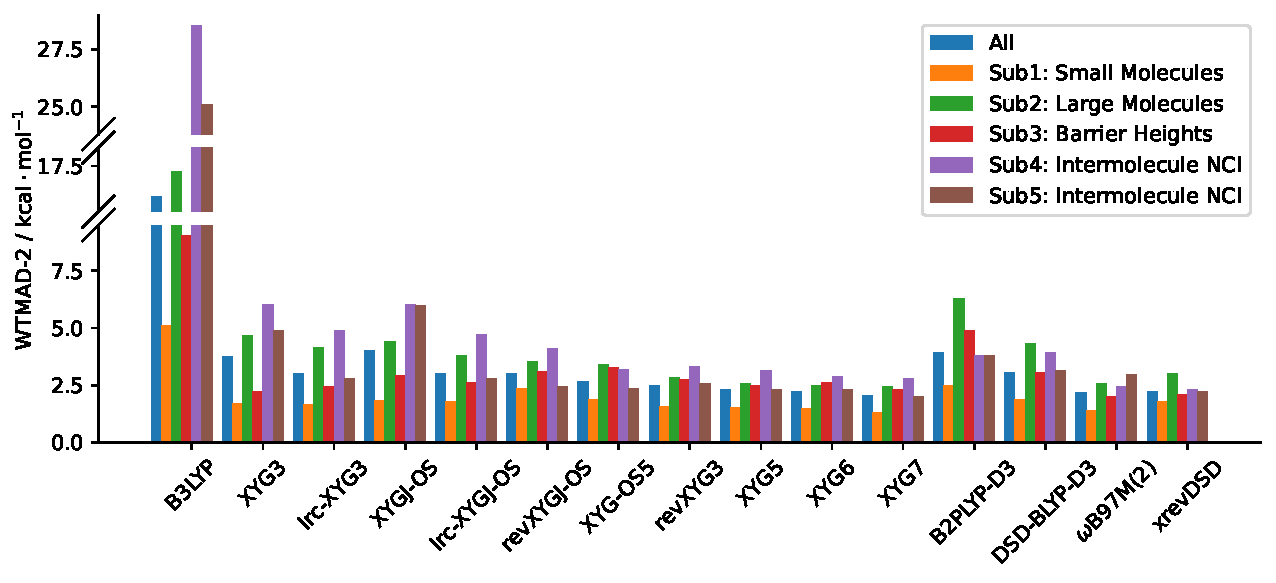
\includegraphics[width=0.8\textwidth]{assets/xdh-b3lyp-wtmad.pdf}
  \caption[双杂化泛函对 GMTKN55 数据集的测评]{各类双杂化密度泛函与 B3LYP 杂化泛函在 GMTKN55 数据集上的 WTMAD-2 测评表现。数据取自文献\cite{Zhang-Xu.JPCL.2021}。图表样式参考论文\cite{Yan.Thesis.2022}。下图中的 xrevDSD 泛函指代 xrevDSD-PBEP86-D4。}
  \label{fig.1.xdh-b3lyp-wtmad}
\end{figure}

\textbf{固体能量测评表现}。图 \ref{fig.1.xdh-solid} 中,王艺臻、李亚静等对 XYG3、XYGJ-OS 双杂化泛函、以及部分低阶 (2--4 阶) 泛函作分子解离能与固体聚合能的测评\cite{Wang-Xu.JA.2021}。其中,CE14 测试集包括 14 种具有强聚合能 (包括强共价键与离子键) 的固体,Bond142 测试集则是由 142 个小分子的键解离能。测评结果表明。尽管 SCAN 与 SCAN0 在处理固体聚合能上有不亚于 xDH 的测评结果,但在分子键能问题上则没有很好的表现。XYG3 与 XYGJ-OS 可以相比于其他低阶泛函、或波函数理论下的 MP2 与 RPA 方法,能够更好地同时处理固体与分子体系中强共价作用的问题,取得两家之长。该工作的其它测评表明,XYGJ-OS 在金红石的两相结构、一氧化碳分子在氯化钠晶体下的吸附能等典型固体计算问题下也有优异的表现。

\begin{figure}[h]
  \centering
  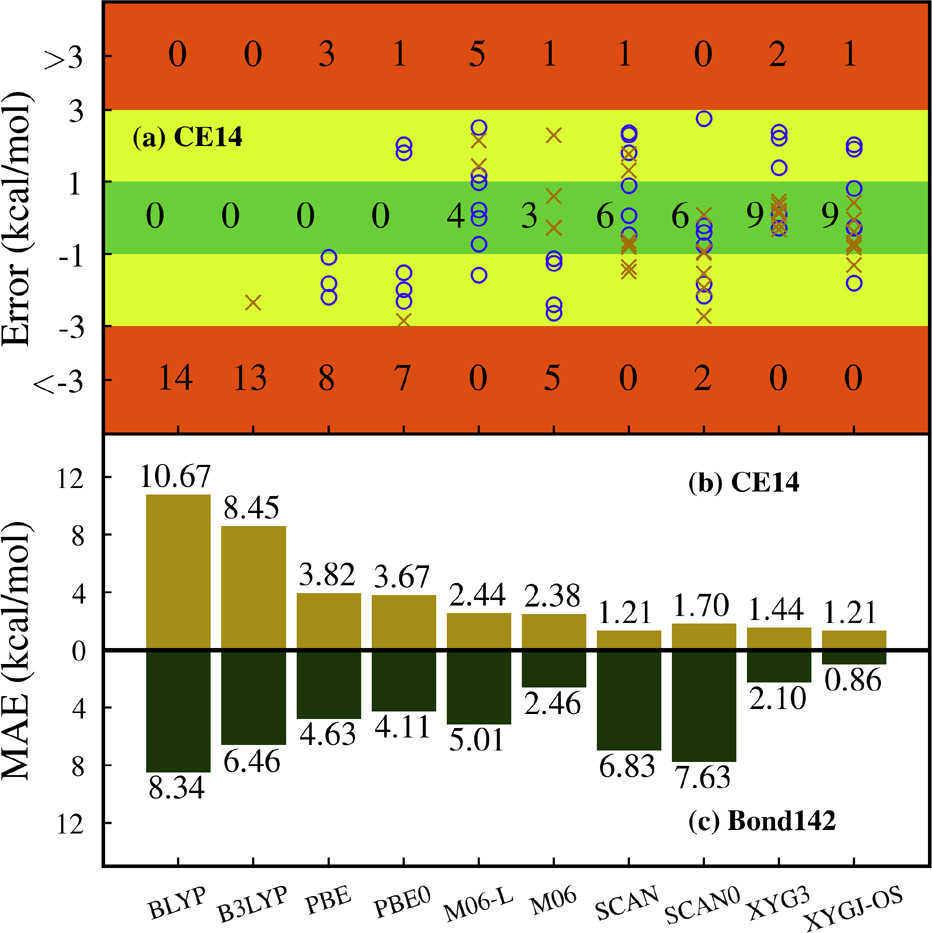
\includegraphics[width=0.4\textwidth]{assets/xdh-solid.jpeg}
  \caption[泛函近似对固体聚合能与分子键解离能问题的测评]{固体聚合能测试集 CE14 与分子键解离能测试集 Bond142 测评结果。CE14 呈现的是分摊到每个原子上的误差表现。图片取自文献\cite{Wang-Xu.JA.2021}。}
  \label{fig.1.xdh-solid}
\end{figure}

\textbf{分子几何结构}。图 \ref{fig.1.xdh-pbe0-bond} 中,苏乃强等对包括 xDH 型双杂化泛函的部分杂化、双杂化泛函作分子几何结构的测评\cite{Su-Xu.SCC.2013}。为了方便比较测评结果,选取了缩放的 s-MAD (即以 XYG3 为单位测评结果作为 1 进行缩放的平均绝对值误差) 作为测评依据。其中,Cov 测试集包括 63 种共价分子与离子体系、NBI 测试集选用了 6 种小分子的二聚体结构用于测评非共价相互作用下的键长表现、TS 测试集收录了 12 个过渡态结构信息。可以看到,作为“Jacob 阶梯”第 5 阶的双杂化泛函的总体表现明显优于第 4 阶的 B3LYP 与 PBE0。除了 xDH-PBE0 在非键作用体系有待改进外,xDH 型泛函在各个数据集上的表现也明显优于 B2PLYP 或 MP2。

\begin{figure}[h]
  \centering
  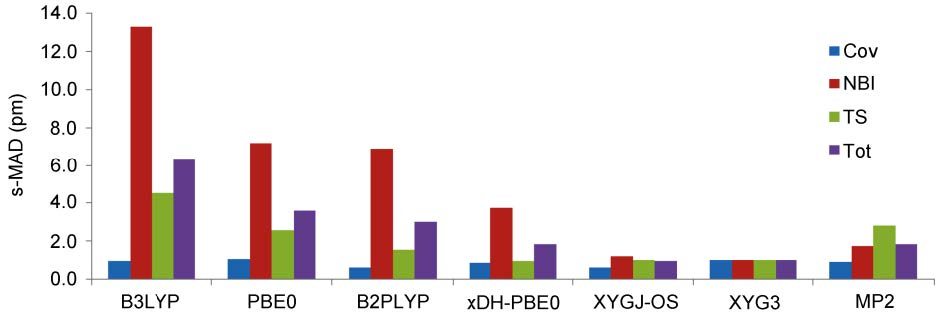
\includegraphics[width=0.7\textwidth]{assets/xdh-pbe0-bond.jpg}
  \caption[泛函近似对分子构型问题的测评]{部分杂化、双杂化泛函及 MP2 方法在分子结构上的总体表现。Cov 代表共价键合分子、NBI 代表非键作用体系、TS 代表过渡态结构、Tot 代表三者的平均。图片取自文献\cite{Su-Xu.SCC.2013}。}
  \label{fig.1.xdh-pbe0-bond}
\end{figure}

\textbf{振动频率}。表 \ref{tab.1.xdh-freq-bench} 中,谷永浩等对部分泛函的谐振频率作测评\cite{Gu-Xu.JCTC.2021}。测试集 F38 包含 38 个小分子的高精度谐振频率实验测量结果 (除 \ce{NH3} 的伞式振动参考值为 CCSD(T)/cc-pVQZ 计算结果)。XYGJ-OS、B2PLYP、xDH-PBE0 的测评表现较好,与实验结果的误差平均不超过 30 $\text{cm}^{-1}$。与此同时,XYGJ-OS 的误差分布较窄,产生较大误差的分子很少。对比 xDH 中表现较好的泛函 XYGJ-OS 与 xDH-PBE0、与其基底泛函 B3LYP 与 PBE0,可以认为在频率计算问题中,泛函的精度仍然沿着“Jacob 阶梯”的爬升稳步提高。

\begin{table}[h]
\centering
\caption[泛函近似对分子谐振频率问题的测评]{部分泛函在 F38 测试集下谐振频率计算的测评表现。误差单位为波数 ($\text{cm}^{-1}$)。数据取自文献\cite{Gu-Xu.JCTC.2021}。}
\label{tab.1.xdh-freq-bench}
\widetabular{
  \begin{tabular}{l
      S[table-format=+3.1]
      S[table-format=+3.1]
      S[table-format=+3.1]
      S[table-format=+3.1]
      S[table-format=+3.1]
      S[table-format=+3.1]}
    \toprule
        & {XYG3} & {XYGJ-OS} & {xDH-PBE0} & {B2PLYP} & {B3LYP} & {PBE0} \\
    \midrule
    MAD & 42   & 19      & 28       & 18     & 33    & 42   \\
    MIN & -87  & -65     & -105     & -51    & -75   & -55  \\
    MAX & 115  & 42      & 51       & 96     & 130   & 122  \\
    误差范围 & 202 & 107 & 156 & 147 & 205 & 177 \\
    \bottomrule
  \end{tabular}
}{}
\end{table}

\textbf{核磁屏蔽常数}。图 \ref{fig.1.xdh-nmr} 中,颜文杰等对部分双杂化泛函的核磁屏蔽常数作测评\cite{Yan-Xu.JCTC.2022}。FPA-M 数据集包含 20 个分子的 34 个 \ce{^{13}C}、\ce{^{15}N}、\ce{^{17}O}、\ce{^{19}F} 原子核的化学位移理论计算结果;其参考值是 FPA 模型下的 CCSD(T)/CBS 结果。测评表明,XYGJ-OS 在诸多双杂化泛函中有出色的表现,并且误差明显小于 Stoychev 等的测评文章\cite{Stoychev-Neese.JCTC.2018} 中表现最好的 DSD-PBEP86 泛函。该工作同时测评了氢原子的化学位移,表明 XYGJ-OS 与 xDH-PBE0 等泛函在 HC\_48/40 数据集上的测评精度对于 \ce{^{1}H} 而言约为 0.03 ppm、对于 \ce{^{13}C} 而言约为 1 ppm,达到了相当高的精度。

\begin{figure}[h]
  \centering
  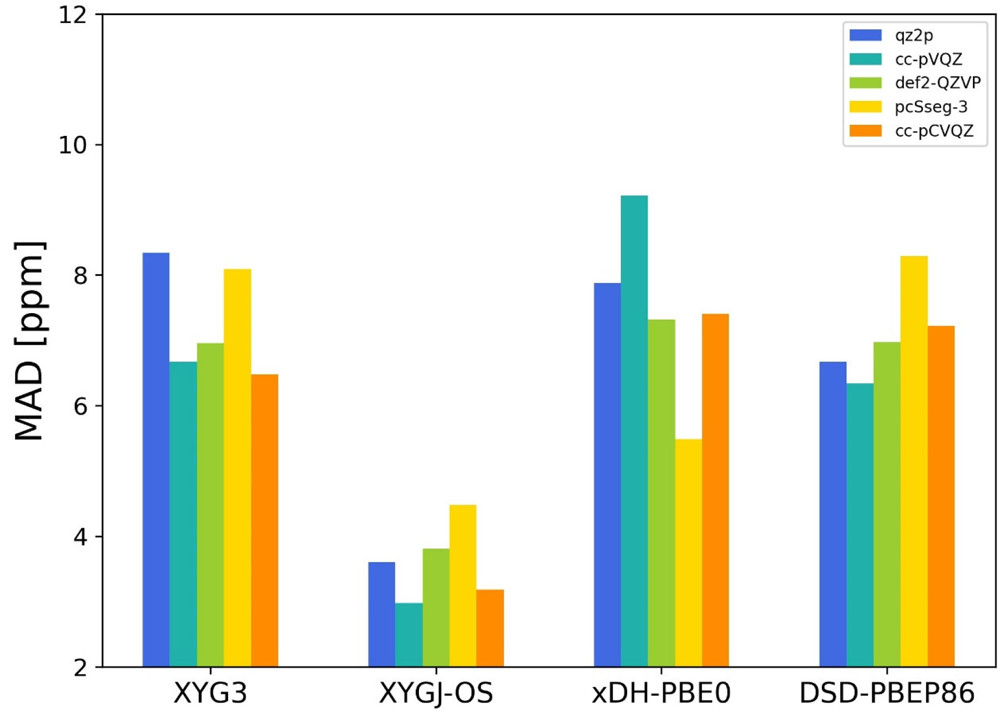
\includegraphics[width=0.4\textwidth]{assets/xdh-nmr.jpeg}
  \caption[泛函近似对 NMR 屏蔽常数问题的测评]{部分双杂化泛函在 FPA-M 集上以 4-$\zeta$ 基组计算的 NMR 屏蔽常数测评表现。图片取自文献\cite{Yan-Xu.JCTC.2022}。}
  \label{fig.1.xdh-nmr}
\end{figure}

\section{本文研究思路与主要工作}

xDH 型泛函构造的理论框架搭建在绝热路径与 G\"{o}rling-Levy 微扰之上,使用较好的单电子轨道作为基础,并在能量计算中追求“Jacob 阶梯”上更高、更精确的阶梯,有着良好的理论基础。xDH 型双杂化泛函在分子能量与性质计算上,其精度水平代表了目前密度泛函方法的最高水准。对于类如 MP2 与 RPA 等相近计算量或计算标度的 post-SCF 方法而言,双杂化泛函的精度通常也更为优异。近年来发展的 xDH 泛函在主族化学反应的能量的表现,已经在切实地逼近 1 kcal/mol 的化学精度;而其它性质的测评工作也表明,xDH 型泛函不仅在能量,还在分子几何结构、振动频率、核磁屏蔽常数等问题上有令人鼓舞的表现。而这些良好的数值结果,也印证了 xDH 型泛函良好的理论框架的重要性。但也需要指出,目前发展的大多数 xDH 型泛函近似的具体实现,依赖于 (Generalized) Kohn-Sham 框架导出的轨道、以及 MP2 型相关能;这两者存在的问题,也可能会反映到 xDH 型双杂化泛函、以及作为退化形式的 bDH 型双杂化泛函的测评表现中。

除了精度上双杂化泛函仍然有发展空间外,其在应用的推广也是重要的课题。在双杂化泛函刚提出的 2004--2010 年代,由于大多数计算化学软件在处理 MP2 型相关能时的计算量很大;即使测评结果较好,也难以推广到实际的应用中。随着一系列针对相关能以及双电子积分计算近似方法、算法与程序的发展,在处理 20 原子以下的分子体系时,MP2 相关能的计算耗时经常少于自洽场的计算耗时,使得双杂化泛函在能量计算问题上不再有严重的效率瓶颈。而对于更大的计算体系,ONIOM 或 XO 等组合化学方法通常可以有效地拆分问题而不严重影响计算精度\cite{Guo-Xu.JCC.2012, Chen-Xu.JCTC.2020, Chen-Xu.NC.2023}。因此,在可见的未来内,在分子体系的计算问题上,双杂化密度泛函的主要应用会集中在数十个原子左右尺度的问题上。

基于以上的研究思路和认识,本文的主要工作从以下五个方面展开。
\begin{enumerate}[nosep]
  \item \textbf{基于成对电子方法的双杂化能量泛函实现与测评。}(第 \alertref{sec.2.title} 章) MP2 型相关能在处理分子解离曲线、过渡金属体系等涉及 Kohn-Sham 轨道能级近简并问题时,容易导致及其严重的误差。为减小近简并体系误差的严重性,双杂化泛函中需要考虑引入其它形式的相关能。基于 G\"orling-Levy 微扰所构建的密度泛函与波函数理论的桥梁,本工作尝试在双杂化泛函中,引入以波函数理论中对 MP2 相关能矫正方法 MP2/cr\cite{Dykstra-Davidson.IJQC.2000} 为代表的成对电子型相关能。我们将构建新的泛函参数化模型,并对参数作系统的优化,考察该类型泛函在一般双杂化泛函表现优异的主族化学反应、与表现欠佳的多参考体系和解离分子体系下的表现。我们期望这份工作,在双杂化近似的框架下,向真实泛函迈进一小步。

  \item \textbf{双杂化泛函的电性质梯度理论与程序实现。}(附录 \alertref{sec.3.title}) 许多分子的性质,譬如分子频率、偶极矩与极化率、化学屏蔽常数、弛豫密度等都需要基于梯度理论得以计算实现。xDH 型泛函的一阶梯度与二阶梯度已经分别由苏乃强等\cite{Su-Xu.SCC.2013}与谷永浩等\cite{Gu-Xu.JCTC.2021}提出。作为本工作中后三章内容的程序实现基础,在电性质外场为微扰的前提下,对 DH 的梯度理论作回顾。除此之外,本工作将尝试扩充该梯度理论到更为一般的非变分双杂化泛函框架,为将来在同一程序框架下实现多种形式的双杂化泛函能量与梯度性质作准备。最后,作为该框架的具体应用,我们将基于开源框架 \textsc{PySCF} 发展扩展程序 \textsc{dh},实现 RI 近似下包含 MP2 型相关能的 DH 极化率,以扩展目前 DH 在分子性质上的算力到 2000 以上基函数的级别。这部分工作仅程序实现是独立完成的工作;理论部分是前人工作的重新推演与整理,{\color{red}\textbf{并非独创性工作}},且由于较为冗长,因此置于附录。
  
  \item \textbf{双杂化泛函原子体系电子云密度与能量测评。}(第 \alertref{sec.4.title} 章) Medvedev 等指出,在非常基本的原子体系能量与密度计算问题上,密度泛函近似并没有随着提出的年代愈近有更好的表现\cite{Medvedev-Lyssenko.S.2017};这让该文章作者产生了“密度泛函是否偏离了逼近真实泛函的道路上”的疑问。他们同时指出,表现欠佳的泛函的共性是含有重度的参数拟合、以及没有建立在合理的理论模型之上或泛函近似在“Jacob 阶梯”的阶数较低。本工作在 Medvedev 等人的测评基础上,对诸多双杂化泛函进行原子能量与密度的计算测评。我们将探究以 xDH 型泛函为代表的双杂化泛函,作为少或无拟合参数、且不专门针对原子体系进行优化的泛函,是否有着相当良好的测评表现;以及随着密度泛函近似的“Jacob 阶梯”的提升,密度泛函是否在原子体系问题下精度有精度的改善。
  
  \item \textbf{高精度基组外推方法在 CCSD(T) 静态极化率计算上的应用。}(第 \alertref{sec.5.title} 章) 该部分工作是第 \alertref{sec.6.title} 章测评双杂化泛函静态极化率的前置工作。静态极化率是描述光学性质与分子间相互作用等问题的重要物理量。一般来说,静态极化率的实验精度误差为 0.5\% 左右;但目前大多数测评数据集的参考值在计算方法或基组上,都与该精度级别有一定差距。有赖于当前高效率的双杂化泛函的极化率程序,大基组的 MP2 极化率对计算资源的消耗已比较小;但可以作为极化率参考值计算方法的 CCSD(T) 计算消耗仍然巨大。FPA 方法是一种波函数理论的组合方法;在我们的工作中,它将大基组的 MP2 计算结果与中等基组大小的 CCSD(T) 相关能结果结合起来,从而以较低的计算代价实现高精度的极化率计算。本工作将系统地测评各级别 FPA 方法的误差,并将 FPA 方法应用到现有的极化率数据集,以提升数据集精度。
  
  \item \textbf{双杂化泛函的静态极化率测评。}(第 \alertref{sec.6.title} 章) 本工作对目前流行的 MP2 型双杂化泛函作系统性的静态极化率测评。该测评的结果将表明,xDH 型泛函在无机与有机、自旋极化与非极化、小分子与中等分子等各类体系下,都有非常良好的极化率表现。该工作也尝试从长短程分离、自旋相同与相反、泛函拟合参数等方面切入,考察这些效应对双杂化泛函在极化率测评表现上的影响。
  
\end{enumerate}
从章节编排上,摘要的介绍顺序是程序与数据集等基础的发展 (附录 \alertref{sec.3.title}、第 \alertref{sec.5.title} 章),泛函开发 (第 \alertref{sec.2.title} 章),泛函测评 (第 \alertref{sec.4.title}、\alertref{sec.6.title} 章)。正文的介绍顺序是能量计算问题 (第 \alertref{sec.2.title} 章),作为第 \alertref{sec.4.title}、\alertref{sec.5.title}、\alertref{sec.6.title} 章的技术支撑的程序开发 (附录 \alertref{sec.3.title}),作为一阶性质的电子云密度测评 (第 \alertref{sec.4.title} 章),作为第 \alertref{sec.6.title} 章的参考值支撑的高精度组合方法开发 (第 \alertref{sec.5.title}),作为二阶性质的极化率测评 (第 \alertref{sec.6.title} 章)。

\newpage



%-----后置区-----

% 后置部分包含参考文献、声明页(自动生成)等
\backmatter

% 打印参考文献列表
\printbibliography

\end{document}
